\documentclass[aspectratio=169,10pt]{beamer}

\usepackage[utf8]{inputenc}

\usepackage{multicol}
\usepackage{multirow}
\usepackage{textcomp} % to use \textmu
\usepackage[absolute,overlay]{textpos} % to place floating text boxes with \begin{textblock*}{width}(x,y)
\usepackage{tcolorbox}

\usepackage{tikz}
\usetikzlibrary{decorations.pathreplacing}

\usepackage{graphicx}
\graphicspath{{./figuras/}}

\setbeamertemplate{navigation symbols}{}

\title[Fabricación CMOS]{Proceso de Fabricación CMOS}
\subtitle{}
\author[Dr.-Ing. Juan José Montero-Rodríguez]{Dr.-Ing. Juan José Montero-Rodríguez}
\institute[]{Instituto Tecnológico de Costa Rica\\Escuela de Ingeniería Electrónica\\Elementos Activos}
\date{Semestre I-2019}
\titlegraphic{
\includegraphics[height=8mm]{logoTEC.png}}


\begin{document}

\begin{frame}
\titlepage
\end{frame}


\begin{frame}
\frametitle{Objetivos}

\textbf{Principios de fabricación de circuitos integrados (2.5 semanas)}

\begin{itemize}
	\item El proceso de fabricación CMOS: materiales, técnicas y flujo de fabricación, prevención de efecto de enganche
	\item Integración de elementos pasivos, capacitores conmutados para integración de resistencias.
	\item Principios de layout e introducción al flujo de back-end
\end{itemize}
\end{frame}


\begin{frame}
\frametitle{Fabricación de Circuitos Integrados}
\centering
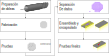
\includegraphics[width=12cm]{fabIC}
\end{frame}


\begin{frame}
\frametitle{Técnicas de Fabricación}
Las principales técnicas para fabricación de circuitos integrados son:

\begin{itemize}
	\item Obtención de silicio cristalino
	\item Oxidación térmica
	\item Litografía
	\item Dopado
	\item Deposición
	\item Decapado
\end{itemize}
\end{frame}


\begin{frame}
\frametitle{Obtención de Silicio Ultrapuro}
\centering

\includegraphics[width=11cm]{obleas}
\end{frame}


\begin{frame}
\frametitle{Obtención de Lingotes de Si Cristalino}

\begin{columns}
\begin{column}{0.4\textwidth}
Dos métodos:

\begin{itemize}
	\item Método de Czochralski
	\item Método de Zona Flotante
\end{itemize}
	
\vspace{5mm}
Método de Czochralski:

\begin{itemize}
	\item Derretir silicio policristalino y mantenerlo a T $<$ 1417 $^\circ$C
	\item Introducir un cristal semilla
	\item Controlar el crecimiento del lingote por medio de la velocidad de extracción, temperatura de fusión y velocidad de rotación	
\end{itemize}
\end{column}
\begin{column}{0.5\textwidth}
	\centering
	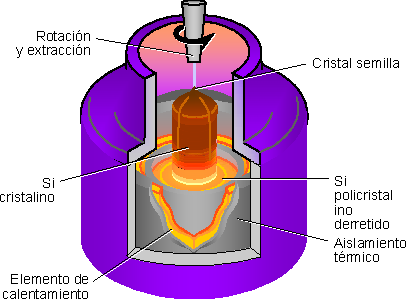
\includegraphics[width=8cm]{czochralski}
\end{column}
\end{columns}
\end{frame}


\begin{frame}
\frametitle{Obtención de Lingotes de Si Cristalino}
\centering
\begin{columns}
	\begin{column}{0.5\textwidth}
		\centering
		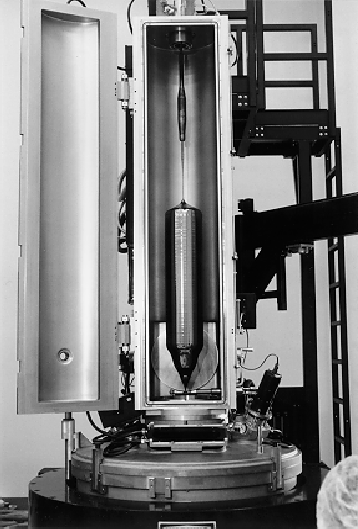
\includegraphics[width=5cm]{czochralski2}
	\end{column}
	\begin{column}{0.5\textwidth}
		\centering
		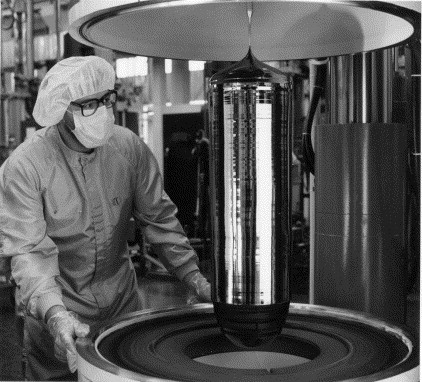
\includegraphics[width=7cm]{czochralski3}
	\end{column}
\end{columns}
\end{frame}


\begin{frame}
\frametitle{Obtención de Lingotes de Si Cristalino}

\begin{columns}
	\begin{column}{0.5\textwidth}
		Método de Zona Flotante
		
		\begin{itemize}
			\item Lingote de Si policristalino de alta pureza
			\item Inductor calienta una zona del lingote y lo derrite
			\item Impurezas se difunden del sólido al líquido, dejando el sólido purificado
		\end{itemize}
	
	\centering
	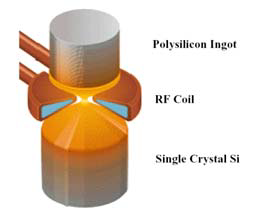
\includegraphics[width=5cm]{floating1}
	\end{column}
	\begin{column}{0.5\textwidth}
		\centering
		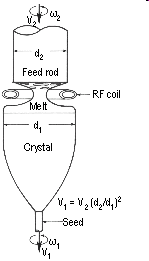
\includegraphics[width=4cm]{floating2}
	\end{column}
\end{columns}
\end{frame}


\begin{frame}
\frametitle{Obtención de Obleas}

\begin{columns}
	\begin{column}{0.5\textwidth}

		\begin{itemize}
			\item Corte de flat grind
			\item Corte de obleas
			\item Identificación de oblea
			\item Decapado químico
			\item Pulido
			\item Limpieza de la superficie
		\end{itemize}
	
	\centering
	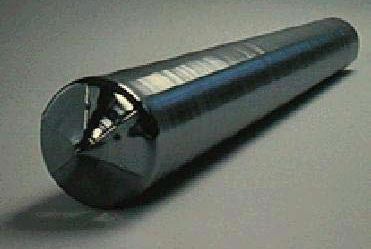
\includegraphics[width=5.5cm]{wafer}
	\end{column}
	\begin{column}{0.5\textwidth}
		\centering
		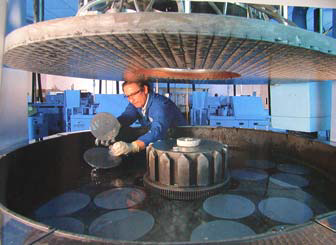
\includegraphics[width=6.5cm]{wafer2}
		
		\raggedright
		\begin{itemize}
			\item Preparación de superficie con pulido químicomecánico
			\item (CMP, chemical mechanical polishing)
		\end{itemize}
	\end{column}
\end{columns}
\end{frame}


\begin{frame}
\frametitle{Oxidación Térmica}
\begin{columns}
\begin{column}{0.75\textwidth}
	Creación de capas de óxido
	
	\vspace{3mm}
	Hornear las obleas en un horno de alta temperatura 
	
	(900 $^\circ$C $<$ T $<$ 1200 $^\circ$C) en presencia de oxígeno o agua
	
	\vspace{5mm}\centering
	Si + O\textsubscript{2} $\rightarrow$ SiO\textsubscript{2} (oxidación seca)
	
	\vspace{3mm}
	O bien
	
	\vspace{3mm}
	Si + 2H\textsubscript{2}O $\rightarrow$ SiO\textsubscript{2} +H\textsubscript{2} (oxidación húmeda)
	
	\vspace{5mm}\raggedright
	El tiempo de oxidación y la temperatura determinan el espesor de la capa de óxido
	
	\vspace{3mm}
	Oxidación seca produce óxido de mejor calidad
\end{column}
\begin{column}{0.25\textwidth}
	\centering
	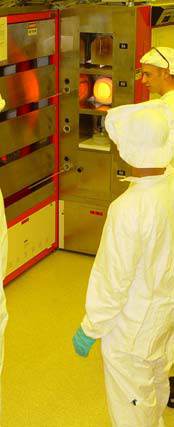
\includegraphics[width=3cm]{thermalSiO2}
\end{column}
\end{columns}
\end{frame}


\begin{frame}
\frametitle{Litografía}
\begin{columns}
\begin{column}{0.4\textwidth}
Litografía:

Creación de patrones para alterar o moldear la forma existente de una capa de material depositado.

\vspace{5mm}
Se realiza con ayuda de una máscara o retícula que transmite el patrón a la capa por moldear. La máscara sirve de “negativo” del patrón a transferir.

\vspace{5mm}
Fotoresistencia: 

Material que cambia su solubilidad al contacto con la luz
\end{column}
\begin{column}{0.6\textwidth}
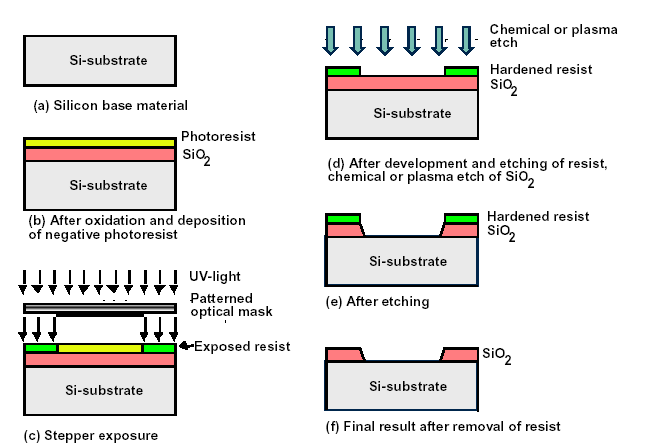
\includegraphics[width=9cm]{lithography}
\end{column}
\end{columns}
\end{frame}


\begin{frame}
\frametitle{Decapado}
\centering
Alterar o moldear la forma existente de una capa de material depositado

\vspace{4mm}Consiste en remover selectivamente el material depositado según el patrón establecido con ayuda de la litografía

\vspace{4mm}
\begin{columns}
\begin{column}{0.45\textwidth}
	\centering
	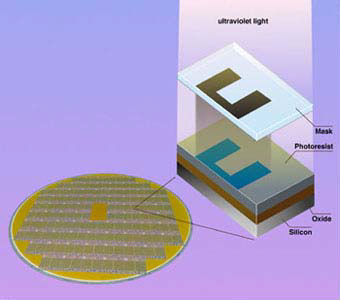
\includegraphics[width=5.75cm]{decapado1}
\end{column}
\begin{column}{0.1\textwidth}
	\centering
	$\Rightarrow$
\end{column}
\begin{column}{0.45\textwidth}
Decapado por bombardeo de iones

Decapado químico = decapado húmedo

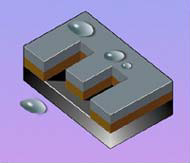
\includegraphics[width=5cm]{decapado2}
\end{column}

\end{columns}
\end{frame}


\begin{frame}
\frametitle{Dopado por Difusión}
Fuente de dopantes: son óxidos en forma sólida, líquida o gaseosa

\begin{itemize}
\item El contacto del silicio con el dopante a altas temperaturas (900 $^\circ$C $<$ T $<$ 1200 $^\circ$C) provoca una reacción en la superficie del silicio, creando una capa de material altamente dopado.
\item Los dopantes se difunden a partir de esta capa hacia la oblea
\end{itemize}

\centering
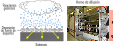
\includegraphics[width=14cm]{doping-diff}
\end{frame}


\begin{frame}
\frametitle{Dopado por Implantación}
Implantación iónica: gas dopante se ioniza y se acelera contra la superficie de la oblea, implantando los átomos dopantes.

\begin{itemize}
\item La profundidad de penetración depende de la energía de implantación. 
\item Después de la implantación, la oblea se calienta para activar la difusión de los dopantes.
\end{itemize}

\centering
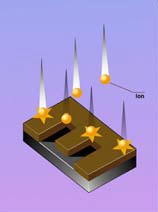
\includegraphics[height=6cm]{doping-impl1}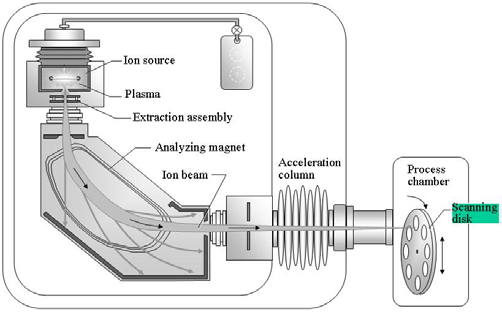
\includegraphics[height=6cm]{doping-impl2}
\end{frame}


\begin{frame}
\frametitle{Difusión vs. Implantación}
\centering

\includegraphics[width=14cm]{diff-vs-imp}
\end{frame}


\begin{frame}
\frametitle{Deposición}
Deposición de capas de material por métodos químicos o físicos

\vspace{4mm}
\centering

\includegraphics[width=13cm]{CVD}
\end{frame}


\begin{frame}
\frametitle{Pruebas}
\begin{columns}
\begin{column}{0.5\textwidth}
	\centering
	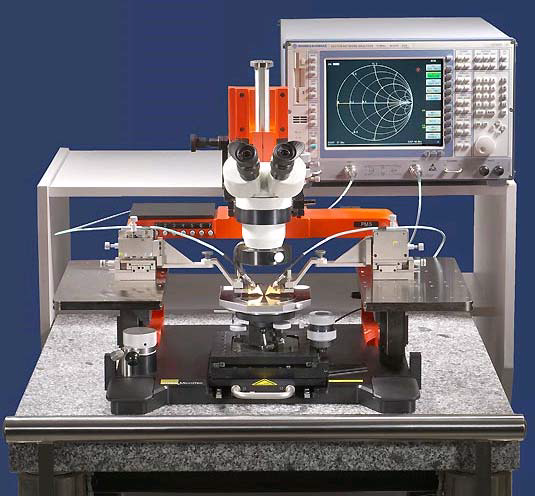
\includegraphics[width=7cm]{probestation}
\end{column}
\begin{column}{0.5\textwidth}
	\centering
	Pueden hacerse a nivel de oblea o a nivel de circuitos encapsulados
	
	\vspace{3mm}
	Se descartan dados defectuosos y se diagnostican fallas de fabricación
	
	\vspace{5mm}
	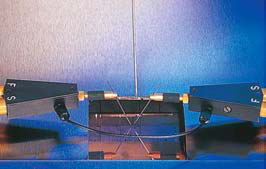
\includegraphics[width=7cm]{probeheads}
\end{column}

\end{columns}
\end{frame}


\begin{frame}
\frametitle{Sección Transversal de Proceso CMOS de Dos Tinas}
\centering
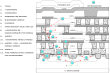
\includegraphics[width=11cm]{CMOS-process}
\end{frame}


\begin{frame}
\frametitle{Sección Transversal de un Procesador AMD}
\centering
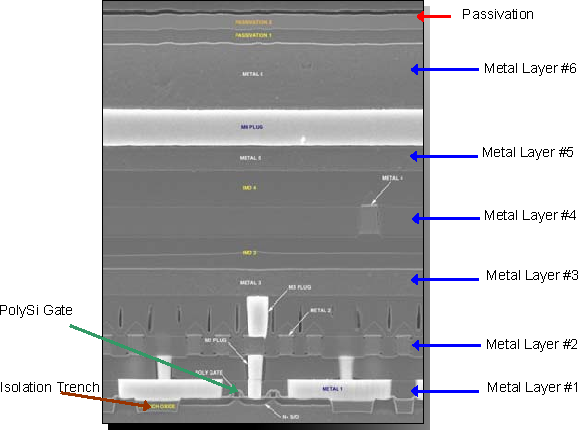
\includegraphics[width=9cm]{AMD}
\end{frame}


\begin{frame}
\frametitle{Proceso de Fabricación CMOS (2 tinas)}
\centering
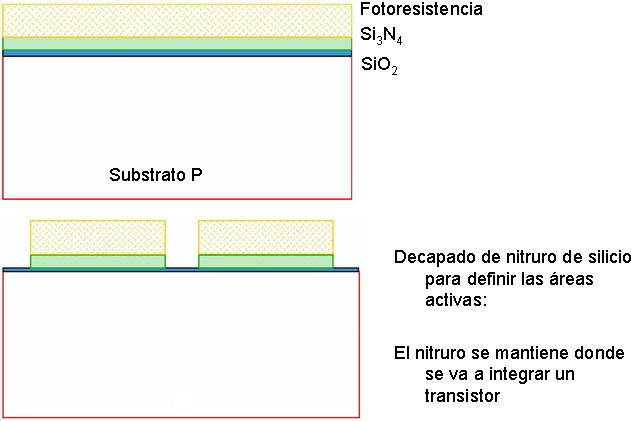
\includegraphics[width=11cm]{CMOS1}
\end{frame}


\begin{frame}
\frametitle{Proceso de Fabricación CMOS (2 tinas)}
\centering
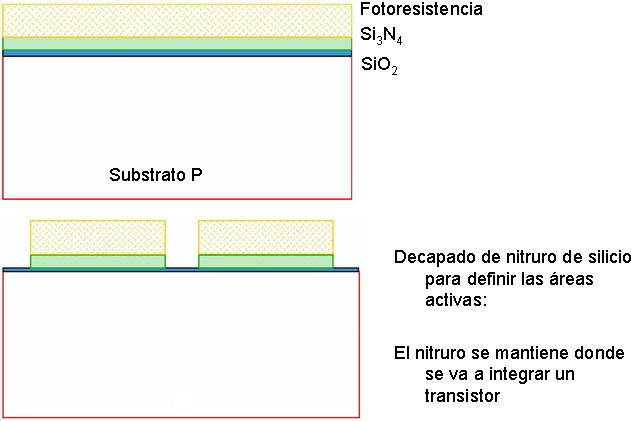
\includegraphics[width=11cm]{CMOS1}
\end{frame}


\begin{frame}
\frametitle{Proceso de Fabricación CMOS (2 tinas)}
\centering
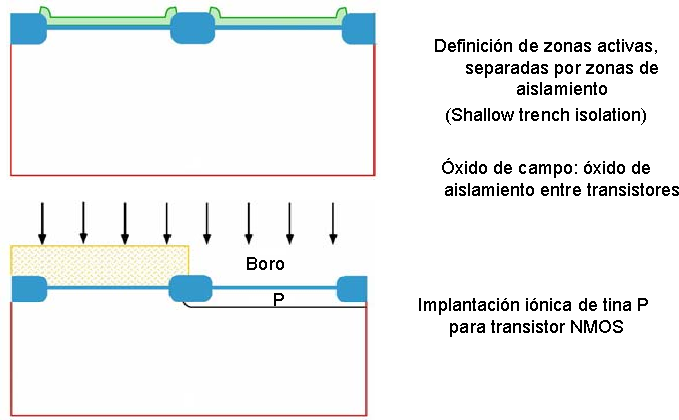
\includegraphics[width=11cm]{CMOS2}
\end{frame}


\begin{frame}
\frametitle{Proceso de Fabricación CMOS (2 tinas)}
\centering
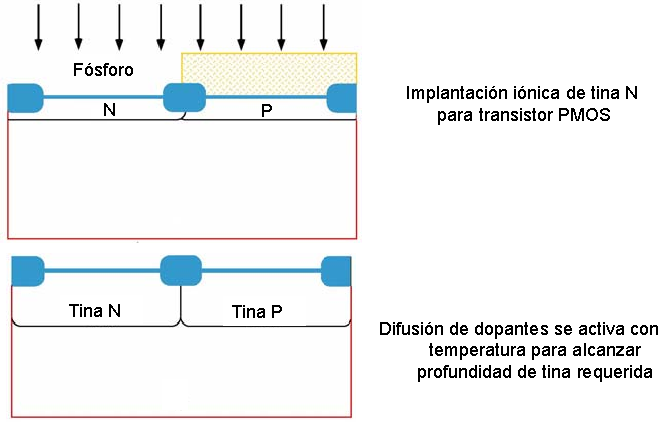
\includegraphics[width=11cm]{CMOS3}
\end{frame}


\begin{frame}
\frametitle{Proceso de Fabricación CMOS (2 tinas)}
\centering
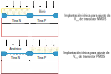
\includegraphics[width=11cm]{CMOS4}
\end{frame}

\begin{frame}
\frametitle{Proceso de Fabricación CMOS (2 tinas)}
\centering
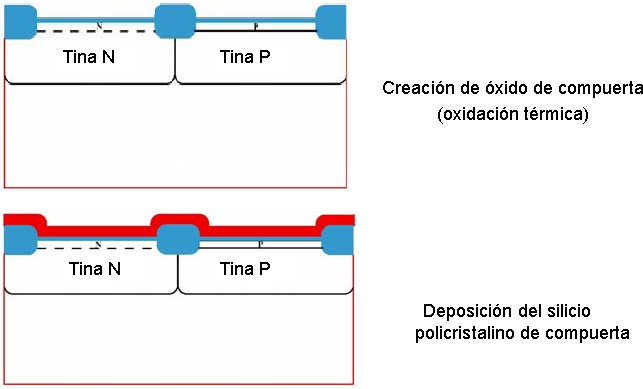
\includegraphics[width=11cm]{CMOS5}
\end{frame}


\begin{frame}
\frametitle{Proceso de Fabricación CMOS (2 tinas)}
\centering
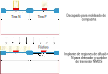
\includegraphics[width=11cm]{CMOS6}
\end{frame}


\begin{frame}
\frametitle{Proceso de Fabricación CMOS (2 tinas)}
\centering
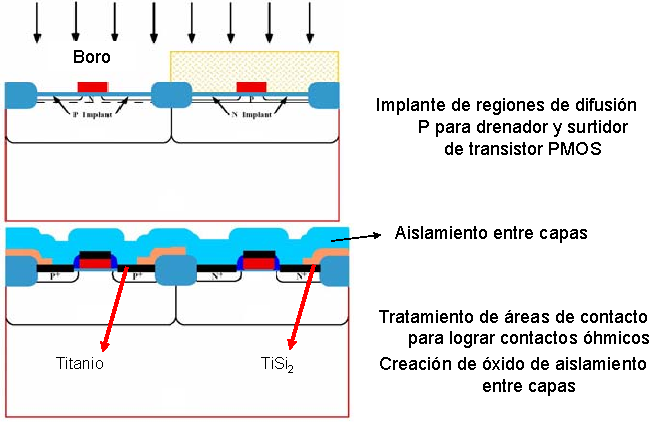
\includegraphics[width=11cm]{CMOS7}
\end{frame}


\begin{frame}
\frametitle{Proceso de Fabricación CMOS (2 tinas)}
\centering
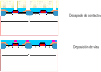
\includegraphics[width=11cm]{CMOS8}
\end{frame}


\begin{frame}
\frametitle{Proceso de Fabricación CMOS (2 tinas)}
\centering
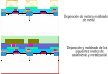
\includegraphics[width=11cm]{CMOS9}
\end{frame}
\end{document}
